\documentclass[margincheck]{withesis}
\usepackage{graphicx}
\usepackage{amssymb,amsmath}
\usepackage{verbatim}
\usepackage{tikz}
\usetikzlibrary{shapes,arrows}

\usepackage{times}
\renewcommand{\ttdefault}{cmtt}

\usepackage{IEEEtrantools}
\usepackage{algpseudocode}
\usepackage{pdflscape}
\usepackage[absolute]{textpos}

\usepackage{fancyhdr}
\setlength{\TPHorizModule}{1in}
\setlength{\TPVertModule}{1in}
\fancypagestyle{lscape}{% 
\fancyhf{} % clear all header and footer fields 
\fancyfoot[LO]{\begin{textblock}{1}(1,   1){\rotatebox{90}{\thepage}}\end{textblock}}
\fancyfoot[LE]{\begin{textblock}{1}(1,10.5){\rotatebox{90}{\thepage}}\end{textblock}}
}
\renewcommand{\headrulewidth}{0pt} 
\renewcommand{\footrulewidth}{0pt}

\usepackage[numbers, sort&compress]{natbib}
\renewcommand{\bibname}{List of References}
\let\oldbibsection\bibsection
\renewcommand{\bibsection}{\oldbibsection\addcontentsline{toc}{chapter}{List of References}\singlespace\raggedright}

\usepackage[bookmarks,
	bookmarksdepth=2,
	pdfauthor={Lewis John Lloyd}, %
	colorlinks, %
	citecolor=black, %
	filecolor=black, %
	linkcolor=black, %
	urlcolor=black]{hyperref}
\usepackage{lipsum}
\usepackage{booktabs}
\usepackage{multirow}

\pagestyle{thesis}
\draftscreen
\setcounter{errorcontextlines}{999}

\DeclareRobustCommand{\BlackBox}{\State \textbf{Black Box: }}
\DeclareRobustCommand{\Test}{\State \textbf{Test: }}
\DeclareRobustCommand{\Define}{\State \textbf{Define: }}
\DeclareRobustCommand{\Update}{\State \textbf{Update: }}
\DeclareRobustCommand{\Set}{\State \textbf{Set: }}
\DeclareRobustCommand{\Calculate}{\State \textbf{Calculate: }}
%\newcommand{\algorithmicset}{\textbf{Set:}}
%\algnewcommand\Solve{\item[\algorithmicset]}
%============================================================================
% commands.tex
%============================================================================
% This file contains:
% 	- Defined Variables
%	- Redefined math shorthand
%	- Defined math shorthand

%============================================================================
% Defined Variables
%============================================================================
% 	- \abstractType:
%		Use: Toggles the type of abstract to be used
%		Default Value: abstract
%		Options: abstract, umiabstract
\newcommand{\abstractType}{abstract}

%============================================================================
% Redefined Math Commands
%============================================================================
% 	- \Vec{1} or \vec{1}
%		Long Name: Vector
%		Arguements[1]: bold and overbar arg1	
\DeclareRobustCommand{\Vec}[1]{%
    \ifmmode
        \mathbf{#1}\,%
    \else
        $\displaystyle \mathbf{#1}\,$%
    \fi
}
\DeclareRobustCommand{\vec}[1]{\Vec{#1}}

\DeclareRobustCommand{\lbm}{%
    \ifmmode
        \text{lb}_{\text{m}}
    \else
        $\displaystyle \text{lb}_{\text{m}}$%
    \fi
}
\DeclareRobustCommand{\lbf}{%
    \ifmmode
        \text{lb}_{\text{f}}
    \else
        $\displaystyle \text{lb}_{\text{f}}$
    \fi
}
\DeclareRobustCommand{\dt}{%
	\ifmmode
		\Delta t
	\else
		$Delta t$
	\fi
}
\DeclareRobustCommand{\dtmax}{%
	\ifmmode
		\Delta t_{\text{MAX}}
	\else
		$\Delta t_{\text{MAX}}$
	\fi
}
\DeclareRobustCommand{\dx}{%
	\ifmmode
		\Delta x
	\else
		$\Delta x$
	\fi
}

\delimitershortfall-1sp
\newcommand\abs[1]{\left|#1\right|}

\tikzstyle{Decision} = [diamond, draw, text width=4.5em, text badly centered, node distance=3cm, inner sep=0pt]
\tikzstyle{Action} = [rectangle, draw,text width=5em, text centered, node distance=3cm, rounded corners, minimum height=0em]
\tikzstyle{NodePoint} = [circle, draw, minimum height = 0 em, node distance = 3 cm]
\tikzstyle{BlackBox} = [rectangle, draw, text centered, node distance=1cm, fill=black!10]
\tikzstyle{line} = [draw, -latex']
    

\begin{document}

\chapter{Introduction}
\label{chap:intro}
In the United States, the goal of Nuclear Power Plant (NPP) designers, builders, operators, and regulators is to ensure the safety of the public during both normal operations and during severe accidents.
It is the responsibility of the Nuclear Regulatory Commission (NRC) to issue licenses for the construction and operation of nuclear reactors.
Chapter 1 of Title 10 of the Code of Federal Regulations (10CFR) details the regulatory procedures that govern the NRC.
Part 50 of 10CFR (10CFR50), lays out the process by which an applicant can obtain both construction and operating licenses for NPPs.
One documents required by 10CFR50 is the a safety analysis report (SAR) prior to the issuance of any license.
Depending upon the particular license being pursued by the applicant, either a Preliminary Safety Analysis Report (PSAR) or a Final Safety Analysis Report (FSAR) is required.
The PSAR is required for the issuance of a site construction license, while the FSAR is required for the issuance of either an operating license or a combined (construction and operating) license.
For reactors that use light water, $H_2 O$, as a primary coolant, Light Water Reactors (LWR), both types of SARs require that the applicant provide an evaluation of their Emergency Core Cooling System (ECCS) during postulated loss-of-coolant accidents (LOCA) and loss-of-offsite-power (LOOP).
This evaluation must conform with section 46 of 10CFR50, which requires that the applicant perform analyses for "a number of postulated loss-of-coolant accidents of different sizes, locations, and other properties sufficient to provide assurance that the most severe postulated loss-of-coolant accidents are calculated."
This requirement necessitates that the designers and operators of NPP possess the ability to model the thermal-hydraulic behavior within the core of a reactor during severe accidents.  
The diverse physical conditions experienced by the reactor during severe accidents necessitates the inclusion of a wide array of physics during safety analyses.
Among the physics of interest are fluid-mechanics, neutron transport, structural mechanics, and radio-chemistry.
For each of these disciplines there are dedicated pieces of software under continual development to improve their predictive capabilities.
The work that follows is concerned with the mathematical formulation and solution of the equations governing the thermal-hydraulic behavior of the reactor core.

All operating commercial reactors within the United States are of a LWR design.
There are two types of LWR designs within the US, pressurized water reactors (PWRs) and boiling water reactors (BWRs).
In both cases, the safety analyses required for licensing necessitates the modeling of water in both its fluid and its gaseous phase.
This fact has driven the development of safety software that can model the behavior of water under a extensive range of thermodynamic states, including multiple-phases.
There are several formulations of the governing conservation equations used to predict the thermal-hydraulic response of the nuclear reactor core to transient plant conditions.

Within the United States, there are several codes that are widely available for simulating the thermal-hydraulic response of a nuclear power plant.
These safety codes can be divided into two large categories: system analysis codes, and sub-channel analysis codes.
While there is a swath of overlap between the capabilities of these two categories, each has its own particular strengths and weaknesses.
The system analysis code often have extensive models available for large components such as steam generators, pumps, valves, containment, etc.
RELAP \cite{RELAP}, TRACE \cite{TRACE}, and MELCOR \cite{Summers1994} are three of the more well known of these system level safety analysis codes.
Other codes have extensive modeling capabilities for in-core heat-transfer and fluid-mechanics: COBRA \cite{Thurgood1983c} and VIPRE are two examples of these sub-channel codes.
In the work that follows, the governing physics and the computational framework of interest will be taken from a variant of the aforementioned COBRA sub-channel analysis code.
%--------------------------------------------------------------------------------------------------------------------------------------------------------------------
%--------------------------------------------------------------------------------------------------------------------------------------------------------------------
%--------------------------------------------------------------------------------------------------------------------------------------------------------------------
%--------------------------------------------------------------------------------------------------------------------------------------------------------------------
%--------------------------------------------------------------------------------------------------------------------------------------------------------------------
%--------------------------------------------------------------------------------------------------------------------------------------------------------------------
%--------------------------------------------------------------------------------------------------------------------------------------------------------------------
\section{Geometry of Interest}
\label{sect:topology}
All commercial NPPs the US are designed so that both core coolant channels and nuclear fuel rods are vertically oriented.
Being that COBRA was developed primarily as a sub-channel analysis tool for these NPPs, there is an assumption that the primary flow direction is in-line with the gravity vector, which will be referred to as the axial flow direction.
The physical core being modeled first needs to be converted into a discrete representation. 

The computational grid used by COBRA is a staggered mesh.
With a staggered mesh, there are continuity volumes and there are momentum"volumes; see \fig{fig:staggered_mesh}.
Thermodynamic variables are defined as constant over the continuity volumes, while mass flow-rates are defined as constant over momentum volumes.
The edges of the continuity volumes align with the center of the momentum cells.
The total number of continuity volumes is $n$ while the number of momentum cells is $n+1$. 

\begin{figure}[ht]
\caption{A staggered mesh.}
\label{fig:staggered_mesh}
\begin{center}
\begin{tikzpicture}
\draw (-3,0) rectangle +(1,5);
\draw (0,-1) rectangle +(1,1) (0,0) rectangle +(1,1) (0,1) rectangle +(1,1) (0, 2) rectangle +(1,1) (0,3) rectangle +(1,1) (0,4) rectangle +(1,1) (0, 5) rectangle +(1,1);
\draw[dashed] (3,-0.5) rectangle +(1,1) (3,0.5) rectangle +(1,1) (3,1.5) rectangle +(1,1) (3, 2.5) rectangle +(1,1) (3,3.5) rectangle +(1,1) (3,3.5) rectangle +(1,1) (3, 4.5) rectangle +(1,1) ;
\draw[dashed] (-3,0) -- (4,0);
\draw[dashed] (-3,5) -- (4,5);
\end{tikzpicture}
\end{center}
\end{figure}

The computational modeling framework involve two primary components: sections and channels.
The total axial length of the problem, $L$, is divided into $M$ blocks, $S_i$, known as sections.
Each section is defined by two bounding elevations and a spatial discretization of that span into $J$ discrete non-overlapping axial segments, $\Delta x_{i,j}$, that represent the axial span of the continuity volumes.
The particular spatial discretization of a given section is independent of the other sections.
A sum of the lengths of each section provides the total axial length of given problem, \eqref{eqn:sections}.

\begin{equation}
\label{eqn:sections}
L = \sum_{i=1}^{M} S_i = \sum_{i=1}^{M}\sum_{j=1}^{J(i)} \Delta x_{i,j}
\end{equation}

Within a given section, channels, $C_{k}$, are defined.
A channel inherits the axial discretization of its parent section.
The number of channels in a given section, $T(i)$, is independent of the number of channels in other sections.
The total number of channels, $K$, within a given problem is defined given by \eqref{eqn:number_of_channels}.

\begin{equation}
\label{eqn:number_of_channels}
K = \sum_{i = 1}^{M} T(i)
\end{equation}

For every channel there is defined a cross-sectional area for each of its continuity volumes, $A_{c_{k,j}}$, and each of its momentum volumes, $A_{m_{k,j}}$.
The total volume of a channel, $\omega_k$, is given by the sum over continuity volumes within that channel, \eqref{eqn:channel_volume}.
The momentum volumes are considered to not contain mass.

\begin{equation}
\label{eqn:channel_volume}
\omega_k = \sum_{j = 1}^{J(k)} \Delta x_{k,j} A_{c_{k,j}}
\end{equation}

The sum of all channel volumes, \eqref{eqn:domain_decomp}, is the total domain volume, $\Omega$.

\begin{equation}
\label{eqn:domain_decomp}
\Omega = \sum \omega_{k}
\end{equation}

While the geometric modeling capabilities of COBRA include the ability to model three dimensional flow, by defining orthogonal flow paths connecting channels, this work will deal only with the subset of problems where the flow is quasi-one-dimensional.

%--------------------------------------------------------------------------------------------------------------------------------------------------------------------
%--------------------------------------------------------------------------------------------------------------------------------------------------------------------
%--------------------------------------------------------------------------------------------------------------------------------------------------------------------
%--------------------------------------------------------------------------------------------------------------------------------------------------------------------
%--------------------------------------------------------------------------------------------------------------------------------------------------------------------
%--------------------------------------------------------------------------------------------------------------------------------------------------------------------
%--------------------------------------------------------------------------------------------------------------------------------------------------------------------
\section{Two-Phase Flow}
\label{sect:two_phase_flow}
The primary use of sub-channel analysis codes is to analysis NPP accidents such as a LOOP or a LOCA.
Since the primary purpose of these simulations determination of fuel integrity, the evaluation of effective core cooling during these accidents is the primary goal.
This necessitates the ability to effectively model the heat-transfer between the coolant and the nuclear fuel. 
COBRA is designed specifically for the evaluation of core cooling in LWRs.
During postulated accidents, the coolant, H$_2$0 can undergo phase-change.
To model the complex phenomena of phase-change, the governing equations for the fluid-mechanics within the core will be those of a multicomponent fluids \cite{Drew1998}.
In particular, they will are a subcategory of two-phase flow \cite{Todreas2011, Stewart1984}.
While a complete derivation of the governing equations of two-phase flow is beyond the scope of this work, a list of the commonly used formulations can be found in \app{app:two_phase_flow}.

\subsection{Assumptions}
\label{subsect:assumptions}

The first simplification for modeling the fluid-mechanics is that the exact geometric shape of the interface between the two phases is not necessary.
Since the exact deterministic behavior of the phasic-interface is not required, the governing equations are subjected to an averaging procedure to produce conservation laws for average quantities.
There are several averaging techniques that have been used to motivate the conservation laws for two-phase flow.
There are spatial, temporal, and ensemble averaging techniques, each of which has their own physical interpretations and mathematical formulation \cite{Drew1998, Todreas2011}.
The particular formulation used in this work is that of spatial averaging, in particular, area averaging.
In the area-averaged formulation, the quantities of interest, $a$ are defined as an average over the cross-sectional flow area, $A$, \eqref{eqn:area_average}.
Since all quantities are area-averaged, the tilde in \eqref{eqn:area_average} will be dropped.

\begin{equation}
\label{eqn:area_average}
\tilde{a} = \frac{1}{A}\int_{A} a \;\mathrm{d}\tilde{A}
\end{equation}

The particular formulation of the two-phase flow equation used in COBRA is commonly referred to as a two-phase three-field formulation. 
To more accurately capture the phenomena of interest during accident scenarios, the liquid and the gaseous phases are each divided into two fields.
The two fields of the liquid phase are a continuous liquid field and an entrained droplet field.
The gaseous phase in composed of a \ncg gas and a water-vapor field. 
This ability to track the different fields within a phase provides two important benefits to safety analysis: the ability to account for the effects of \ncgs on condensation, and the ability to model the impact upon heat transfer by dispersed liquid droplets.

Given the four fields of interest, there are twelve conservation equations, one each for the mass, momentum, and energy of each of the four fields.
These equations allow for a description of the time-dependent behavior of the in-core fluid.
In addition, closure relationships are necessary to describe the interactions between the various fields and their inter-facial transfer terms.
However, additional assumptions are made to reduce the number of required conservation laws and the number of corresponding closure relationships.
The following is a list of assumptions that are made to reduce the complexity of the governing equations.

\begin{itemize}
\item{
Thermodynamic and pressure equilibrium exists between the continuous liquid film and the entrained liquid droplets.
This basis for this assumption is that while the entrained droplets are here being modeled by a separate set of governing equations that those of the continuous liquid field, in reality the droplets are constantly entraining and depositing with the continuous liquid field. 
}
\item{
The liquid and gaseous phases are in pressure equilibrium.
}
\item{
The two gaseous phases are fully mixed and in mechanical equilibrium.
As a result of this assumption, the gases move with the same average velocities and obey Dalton's Law of partial pressures.
However, the gases retains separate thermodynamics states.
}
\item{
The viscous dissipation of momentum in the axial flow direction is neglected.
This assumption also removes the generation of energy via viscous dissipation.
}
\item{
The wall-shear effects of viscosity are accounted for via empirically based friction correlations.
}
\end{itemize}

\subsection{Governing Equations}
\label{subsect:governing_equations}

There are four equations representing the conservation of mass of the \ncg field, the continuous liquid field, the dispersed liquid field, and the water vapor field.

\begin{IEEEeqnarray}{rCl}
\label{eqn:conservation_of_ncg}
\frac{\partial \left(\alpha_g \rho_{ncg}\right) }{\partial t } + \nabla \cdot \left( \alpha_g \rho_{ncg} \vec{u}_g \right) & = & s_{m,ncg} \\
\label{eqn:conservation_of_vap}
\frac{\partial \left(\alpha_g \rho_v \right)}{\partial t } + \nabla \cdot \left( \alpha_g \rho_v \vec{u}_g \right)         & = & \Gamma^{'''} + s_{m,v} \\
\label{eqn:conservation_of_liq}
\frac{\partial \left(\alpha_l \rho_l \right)}{\partial t } + \nabla \cdot \left( \alpha_l \rho_l \vec{u}_l \right)         & = & -(1-\eta)\Gamma^{'''} - S^{'''} + s_{m,l} \\
\label{eqn:conservation_of_ent}
\frac{\partial \left(\alpha_e \rho_l \right)}{\partial t } + \nabla \cdot \left( \alpha_e \rho_l \vec{u}_e \right)         & = & -\eta\Gamma^{'''} + S^{'''}+ s_{m,e}
\end{IEEEeqnarray}

The left hand sides of \eqref{eqn:conservation_of_ncg} -- \eqref{eqn:conservation_of_ent} represent the Lagrangian derivative for the given field.
The terms on the right hand side represent the volumetric inter-field ($S^{'''}$), inter-phase ($\Gamma^{'''}$),  and external ($s_k$) sources or sinks of mass.
Since there are two liquid fields, the net phasic mass transfer between the water-vapor field and the liquid fields, $\Gamma^{'''}$, is apportioned between the continuous liquid field and the dispersed liquid field.

\begin{equation}
\label{eqn:apportionment_of_mass_transfer}
\Gamma^{'''} = \Gamma^{'''}_v = -( \Gamma^{'''}_e + \Gamma^{'''}_l ) =  \eta \Gamma^{'''} + (1 - \eta)\Gamma^{'''} = \Gamma^{'''}
\end{equation}

This division is given by \eqref{eqn:apportionment_of_mass_transfer}, where $\eta$ is an apportionment factor.
The inter-field transfer of mass occurs only between the continuous and dispersed liquid fields, \eqref{eqn:entrainment_deentrainment}.

\begin{equation}
\label{eqn:entrainment_deentrainment}
S^{'''}_l + S^{'''}_e = 0
\end{equation}

Within the conservation of mass equations, several assumptions from \sect{subsect:assumptions} are evident.
The mechanical equilibrium of the \ncg and the vapor fields manifest in a singular velocity for the two fields, $\vec{u}_g$, where the $_g$ subscript denotes the total gaseous phase.
Dalton's Law allows the two gaseous fields to occupy the same volume, thus providing for a singular volume fraction, $\alpha_g$.
The thermodynamic equilibrium of the two liquid fields result in only one liquid density, $\rho_l$.

In addition to the conservation of mass, there are conservation of energy equations for each of the two phases, \eqref{eqn:con_energy_gas} -- \eqref{eqn:con_energy_liq}.

\begin{IEEEeqnarray}{rCl}
\label{eqn:con_energy_gas}
\frac{\partial \left( \alpha_g \{\rho_g h_g\} \right)}{\partial t } + \nabla \cdot \left(  \alpha_g \{\rho_g h_g\} \vec{u}_g \right) & =& \nonumber \\
\Gamma^{'''} h^{'}_v + q^{'''}_{i,v} + q^{'''}_{gl}  + q^{'''}_{wg} + \alpha_g\frac{\partial P}{\partial t} + s_{e,g}  & &\\
\label{eqn:con_energy_liq}
\frac{\partial \left( (1 - \alpha_g) \rho_l h_l \right) }{\partial t } + \nabla \cdot \left( \alpha_l \rho_l h_l \vec{u}_l \right) + \nabla \cdot \left( \alpha_e \rho_l h_l \vec{u}_e \right)& = & \nonumber \\
-\Gamma^{'''} h^{'}_l +  q^{'''}_{i,l} - q^{'''}_{gl}  + q^{'''}_{wl} + (1 - \alpha_g) \frac{\partial P}{\partial t} + s_{e,l}  & &
\end{IEEEeqnarray}

The conservation of energy equations used in this work are formulated such that the conserved quantities are the phasic enthalpies, $\alpha_k \rho_k h_k$.
Under the assumption of thermodynamic equilibrium for the two liquid fields, there is a single liquid enthalpy for the two fields.
The gaseous phasic enthalpy, however, is defined according to \eqref{eqn:gaseous_enthalpy}.

\begin{equation}
\label{eqn:gaseous_enthalpy}
\{\rho_g h_g\} = \rho_v h_v + rho_{ncg} h_{ncg}
\end{equation}

The various terms on the right hand sides of \eqref{eqn:con_energy_gas} and \eqref{eqn:con_energy_liq} are defined as follows.
\begin{itemize}
\item{
$\Gamma^{'''} h^{'}_k$:
 energy transfer due to the phase change of water.
 The effective enthalpies, $h^{'}_k$, are dependent upon the mechanism of phase change.
}
\item{
$q^{'''}_{i,k}$:
energy transfer between the liquid fields and the vapor field.
}
\item{
$q^{'''}_{gl}$:
energy transfer between the liquid fields and the \ncgs.
}
\item{
$q^{'''}_{wk}$:
 energy transfer between solid-structure and a given phase.
}
\item{
$\alpha_k \frac{\partial P}{\partial t}$:
 pressure work done by a given phase $k$.
 The liquid volume fraction is the sum of the continuous and the entrained liquid field's volume fractions.
}
\item{
$s_{e,k}$:
 external source/sink of energy for a given field $k$.
}
\end{itemize}

The conservation of momentum equations, \eqref{eqn:con_mom_liq} -- \eqref{eqn:con_mom_ent}, are expressed in vector notation; however, only axial flow is considered in the current work.
Dalton's Law and the assumed mechanical equilibrium between the two gaseous fields enable the use of a single momentum conservation for the net gaseous phase.

\begin{IEEEeqnarray}{rCl}
\label{eqn:con_mom_liq}
\frac{\partial \left( \alpha_l \rho_l \vec{u}_l \right )}{\partial t } + \nabla \cdot \left( \alpha_l \rho_l \vec{u}_l \vec{u}_l \right) & = & \nonumber \\
 -\alpha_l \nabla P + \alpha_l \rho_l \vec{g} - \vec{\tau}^{'}_{wl} + \vec{\tau}^{'}_{i,gl} - (1 - \eta)\Gamma^{'''}\vec{u}^{'} - S^{'''}\vec{u}^{'} + s_{p,l} & & \\
\label{eqn:con_mom_gas}
\frac{\partial \left( \alpha_g \rho_g \vec{u}_g \right) }{\partial t } + \nabla \cdot \left( \alpha_g \rho_g \vec{u}_g \vec{u}_g \right) & = & \nonumber \\
 -\alpha_g \nabla P + \alpha_g \rho_g \vec{g} - \vec{\tau}^{'}_{wg} - \vec{\tau}^{'}_{i,gl} - \vec{\tau}^{'}_{i,ge} + \Gamma^{'''}\vec{u}^{'} + s_{p,g} & & \\
\label{eqn:con_mom_ent}
\frac{\partial \left( \alpha_e \rho_l \vec{u}_e \right) }{\partial t } + \nabla \cdot \left( \alpha_e \rho_l \vec{u}_e \vec{u}_e \right) & = & \nonumber \\
 -\alpha_e \nabla P + \alpha_e \rho_l \vec{g} - \vec{\tau}^{'}_{wl} + \vec{\tau}^{'}_{i,ge} - \eta \Gamma^{'''}\vec{u}^{'} + S^{'''}\vec{u}^{'} + s_{p,l} & &
\end{IEEEeqnarray}

The $\rho_g$ used in \eqref{eqn:con_mom_gas} is defined by \eqref{eqn:gaseous_density}.

\begin{equation}
\label{eqn:gaseous_density}
\rho_g = \rho_{ncg} + \rho_v
\end{equation}

The material derivative of the fluid momentum is represented by the left hand sides of \eqref{eqn:con_mom_liq} -- \eqref{eqn:con_mom_ent}.
The right hand sides represent various surface, boundary, and body forces that act upon the fluid.
The following a quick description of each term.

\begin{itemize}
\item{
$\alpha_k \nabla P$:
pressure gradient acting on field $k$.
}
\item{
$\alpha_k \rho_k \vec{g}$:
gravity body force acting upon field $k$.
}
\item{
$\vec{\tau}^{'}_{wk}$:
 shear forces from contact between field $k$ and the channel walls. 
}
\item{
$\vec{\tau}^{'}_{i,k_1\,k_2}$:
 shear forces from the interface between fields $k_1$ and $k_2$. 
}
\item{
$\Gamma^{'''}\vec{u}^{'}$:
 momentum contribution from the exchange of mass due to the phase change of water.
 The $\vec{u}^{'}$ term depends upon the net inter-phase transfer of mass.
}
\item{
$S^{'''}\vec{u}^{'}$:
 momentum contribution from the exchange of mass between the two liquid fields.
 The $\vec{u}^{'}$ term depends upon the net inter-field transfer of mass.
}
\item{
$s_{p,k}$:
 external sources/sinks of momentum for field $k$.
}
\end{itemize}

Note that the momentum conservation equations are formulated such that the temporal derivatives are of the conserved quantities, which is referred to as a conservative formulation.
This formulation will be retained during the numerical discretization process.
Other common system analysis codes \cite{TRACE, RELAP} use different non-conservative variants of the above equations for their momentum conservation laws.

It will be useful to refer to the collection of continuous conservation laws, \eqref{eqn:conservation_of_ncg} -- \eqref{eqn:conservation_of_ent}, \eqref{eqn:con_energy_gas} -- \eqref{eqn:con_energy_liq}, and \eqref{eqn:con_mom_liq} -- \eqref{eqn:con_mom_ent}, as a vector of equations.
To accomplish this, \eqref{eqn:conservation_equations} defines such a system.
The vector, $\vec{G}$, represents the full conservation equations minus the temporal derivatives of the conserved quantities.

\begin{equation}
\label{eqn:conservation_equations}
\frac{\partial \left( \vec{y} \right)}{\partial t} = \vec{g}(\vec{y}(t))
\end{equation}

The vector, $\vec{y}$, of conserved quantities is defined in \eqref{eqn:conserved_variables}.

\begin{equation}
\label{eqn:conserved_variables}
\vec{y} = [\alpha_g \rho_{ncg}, \alpha_g \rho_v, \alpha_l \rho_l, \alpha_e \rho_l, \alpha_g \rho_g h_g, (1 - \alpha_g) \rho_l h_l, \alpha_g \rho_g \vec{u}_g, \alpha_l \rho_l \vec{u}_l, \alpha_e \rho_e \vec{u}_e]^{T}
\end{equation}

%--------------------------------------------------------------------------------------------------------------------------------------------------------------------
%--------------------------------------------------------------------------------------------------------------------------------------------------------------------
%--------------------------------------------------------------------------------------------------------------------------------------------------------------------
%--------------------------------------------------------------------------------------------------------------------------------------------------------------------
%--------------------------------------------------------------------------------------------------------------------------------------------------------------------
%--------------------------------------------------------------------------------------------------------------------------------------------------------------------
%--------------------------------------------------------------------------------------------------------------------------------------------------------------------
\section{Numeric Approximations}
\label{sect:numeric_approximation}
The set of conservation laws, \eqref{eqn:conserved_variables}, governing the fluid-mechanics within the geometry of interest do not have a general closed form solution.
As such, a method needs to be selected to numerically approximate their solutions.

\subsection{Spatial Approximations}
\label{subsect:spatial_approx}
In COBRA, the finite-volume method was chosen to discretize the governing equations \cite{LeVeque2002}.
The labeling scheme for the volumes is shown in \fig{fig:vertical_pipe_with_cells}, a segment of a vertical channel.
A continuity volume, $j$, is spatially overlapped by two momentum volumes, $j$ and $j-1$.
Variables are indexed by the mesh on which their conservation equations are defined.
For example, the velocity $u_j$ would be spatially located at center of the momentum volume $j$ and at the boundary between the continuity volumes $j$ and $j-1$.

\begin{figure}[ht]
\caption{Illustration of indexing scheme.}
\label{fig:vertical_pipe_with_cells}
\begin{center}
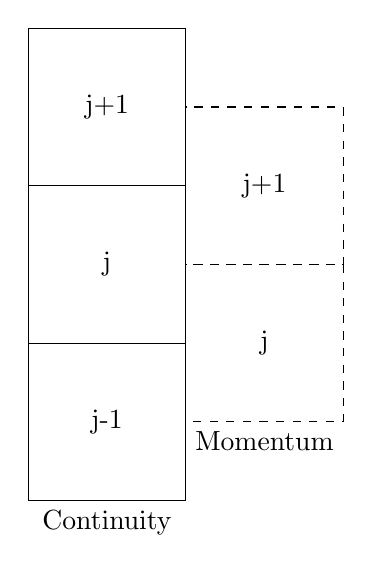
\begin{tikzpicture}
\draw (-2,-3) rectangle +(2,2);
\node[anchor=center] at (-1,-2) {j-1};
\draw (-2,-1) rectangle +(2,2);
\node[anchor=center] at (-1, 0) {j};
\draw (-2, 1) rectangle +(2,2);
\node[anchor=center] at (-1, 2) {j+1};
\draw[dashed] (-0,-2) rectangle +(2,2);
\node[anchor=center] at (1, -1) {j};
\draw[dashed] (-0, 0) rectangle +(2,2);
\node[anchor=center] at (1, 1) {j+1};
\node[anchor=north] at (-1, -3) {Continuity};
\node[anchor=north] at (1, -2) {Momentum};
\end{tikzpicture}
\end{center}
\end{figure}

Recalling the staggered grid from \sect{sect:topology}, the six scalar conservation laws, \eqref{eqn:conservation_of_ncg} -- \eqref{eqn:con_energy_liq}, are each integrated over the continuity volumes.
The assumption in these integrals is that the value of the conserved quantities and all thermodynamically related variables are constant within a given cell.
\fig{fig:constant_value} shows a graphical representation of this idea for a generic function $f(x)$ over several spatial continuity meshes.

\begin{figure}[ht]
\caption{Constant variable values within computational volumes.}
\label{fig:constant_value}
\begin{center}
Picture goes here.
\end{center}
\end{figure}

For illustrative purposes,  the \eqref{eqn:conservation_of_liq} will be integrated over a given volume, $j$, as shown in \fig{fig:single_volume}.

\begin{figure}[ht]
\caption{Single volume over which integration is done.}
\label{fig:single_volume}
\begin{center}
Picture goes here.
\end{center}
\end{figure}

Within a given channel, $k$, a given continuity volume has a constant cross-sectional area, $A_{c_{j}}$, and a length of $\Delta x_{j}$.
The cross-section area of the boundary between two continuity volumes is given by the cross-section area of the momentum volume at that boundary, $A_{m}$.

\begin{IEEEeqnarray}{lcl}
\int_{V_j}\frac{\partial \left(\alpha_l \rho_l \right)}{\partial t } & + & \nabla \cdot \left( \alpha_l \rho_l u_l \right) \mathrm{d}V = \int_{V_j} \left(-(1-\eta)\Gamma^{'''} - S^{'''} + s_{m,l}\right) \mathrm{d}V \nonumber \\
V_j \frac{\partial \left(\alpha_{l,j} \rho_{l,j} \right)}{\partial t } & = & -\int_{V_j}\nabla \cdot \left( \alpha_l \rho_l u_l \right) \mathrm{d}V -(1-\eta_j)\Gamma_j^{'''}V_j - S_j^{'''}V_j + s_{m,l,j}V_j \nonumber \\
V_j \frac{\partial \left(\alpha_{l,j} \rho_{l,j} \right)}{\partial t } & = & -A_{m,j}\left[\alpha_l \rho_l u_l \right]_{x_{j-\frac{1}{2}}}^{x_{j+\frac{1}{2}}} -(1-\eta_j)\Gamma_j^{'''}V_j - S_j^{'''}V_j + s_{m,l,j}V_j \nonumber \\
\label{eqn:spatially_discrete_liq_m_con}
V_j \frac{\partial \left(\alpha_{l,j} \rho_{l,j} \right)}{\partial t } & = & -A_{m,j}\left( <\alpha_l \rho_l>_{d,j+\frac{1}{2}} u_{l,j+1} - <\alpha_l \rho_l>_{d,j-\frac{1}{2}} u_{l,j} \right) \nonumber \\
& & -(1-\eta)\Gamma^{'''}V - S^{'''}V_j + s_{m,l}V_j
\end{IEEEeqnarray}

For the mass-flux terms evaluated on the continuity volume edge, the advected quantity is evaluated using a 1st order upwind method \cite{Tannehill1997}.
The velocity and cross-sectional area utilized in the continuity flux terms, $u_j$ and $A_{m,j}$, have the values defined at the center of the momentum volume that aligns with the edge of continuity volumes.
The sign of the velocity at the volume boundary determines the value of the donored quantity, $<a>_{d,j-\frac{1}{2}}$.
A generic formulation for this scheme is given by \eqref{eqn:upwind_donoring}.
The same general procedure is used for the other five scalar conservation equations.

\begin{equation}
\label{eqn:upwind_donoring}
<a>_{d, j-\frac{1}{2}} = \begin{cases} a_{j-1} &  u_j \geq 0 \\ a_{j} & u_j < 0 \end{cases}
\end{equation}

The three momentum conservation laws, \eqref{eqn:con_mom_liq} -- \eqref{eqn:con_mom_ent}, are integrated over their momentum volume.
The cross section area for a momentum volume, $A_{m,j}$, can be defined independently of the two cross-sectional areas of the adjoining continuity volumes.
The momentum flux terms, \eqref{eqn:momentum_flux_terms}, are treated similarly to the flux terms in the continuity equations.
\begin{equation}
\label{eqn:momentum_flux_terms}
-\min\left(A_{m,j}, A_{m,j+1}\right)\left[<\alpha_l \rho_l u_l>_{d} u_l\right]_{x_{j-\frac{1}{2}}}^{x_{j+\frac{1}{2}}}
\end{equation}
There are two primary differences.
First, the momentum area 
The second difference is that the velocity that is used to determine the origination of the donored quantity is the arithmetic mean of the velocities from the two adjacent momentum volumes, \eqref{eqn:average_advecting_vel}.

\begin{equation}
\label{eqn:average_advecting_vel}
u_{k,j+\frac{1}{2}} = \frac{1}{2}\left(u_{k,j} + u_{k, j+1}\right)
\end{equation}

\subsection{Temporal Approximations}
\label{subsect:temporal_approx}
Once the governing conservation equations have been spatially discretized utilizing the method outlined above, the temporal derivatives need to be numerically approximated.
Using the spatially discrete approximations defined in \sect{subsect:spatial_approx}, the temporally continuous differential equations,\eqref{eqn:conservation_equations}, are now semi-discrete approximations given by \eqref{eqn:temporal_semi_discrete}, where $\vec{G}$ now represents the spatially discrete version of $\vec{g}$.

\begin{equation}
\label{eqn:temporal_semi_discrete}
\frac{\partial \,\vec{y} }{\partial t} = \vec{G}(\vec{y}(t))
\end{equation}

Within COBRA, the temporal derivative is approximated by a one-step difference scheme, \eqref{eqn:simple_partial_t}.
Where the continuous time variables are now evaluated at discrete points, $t^0, t^1, \ldots, t^N$, where $t^0$ represents the initial conditions and $t^N$ represents the final time.
The term one-step refers to the fact that the temporal derivative involves only two consecutive points in time.

\begin{IEEEeqnarray}{rcl}
\int^{t^{n+1}}_{t^n}\frac{\partial \vec{y}}{\partial t}\mathrm{d}\tau & = & \int^{t^{n+1}}_{t^n}\vec{G}(\vec{y})\mathrm{d}\tau \nonumber \\
\vec{y}^{n+1} - \vec{y}^{n} & = & \int_{t^{n+1}}^{t^n}\vec{G}(\vec{y})\mathrm{d}\tau \nonumber  \\
\frac{\vec{y}^{n+1} - \vec{y}^{n}}{\int_{t^{n}}^{t^{n+1}}\mathrm{d} \tau} & = & \frac{\int_{t^{n+1}}^{t^n}\vec{G}(\vec{y})\mathrm{d}\tau}{\int_{t^{n}}^{t^{n+1}}\mathrm{d} \tau} \nonumber \\
\frac{\vec{y}^{n+1} - \vec{y}^{n}}{\Delta t} & = & \frac{\int_{t^{n+1}}^{t^n}\vec{G}(\vec{y})\mathrm{d}\tau}{\int_{t^{n}}^{t^{n+1}}\mathrm{d} \tau} \nonumber \\
\label{eqn:simple_partial_t}
\frac{\vec{y}^{n+1} - \vec{y}^{n}}{\Delta t} & = & \vec{G}(\vec{y}^{*})
\end{IEEEeqnarray}

The choice of how to approximate the temporal-average, $\vec{G}(\vec{y}^{*})$, is a factor that defines the eventual solution algorithm.
The commonly used approximations will be postponed for now. 

\subsection{Nonlinear Approximations}
\label{sect:nonlinear_approximations}

Given the system of discretized PDEs, \eqref{eqn:simple_partial_t}, nine independent parameters are required
Given that there are nine conservation equations, the choice of which nine variables are the independent parameters that will be solved for is another distinguishing characteristic of safety analysis codes.
The choice made in the COBRA sub-channel analysis codes is shown in \eqref{eqn:independent_variables}.

\begin{equation}
\label{eqn:independent_variables}
\vec{x} = [\alpha_{ncg}P_{ncg}, \alpha_g, P, \alpha_e, \alpha_gS h_v, (1 - \alpha_g) h_l, \dot{m}_g, \dot{m}_l, \dot{m}_e]^{T}
\end{equation}

The definition of $\dot{m}_k$ is given by \eqref{eqn:mom_dot}.

\begin{equation}
\label{eqn:mom_dot}
\dot{m}_k = \alpha_k \rho_k u_k A_m
\end{equation}

In the particular discretization utilized, there are several nonlinear terms that are to be evaluated implicitly.

For the two-phase flow equations of interest, the conserved variables at $t^{n+1}$ are nonlinear functions of the independent parameters.
These temporal nonlinearities exist in all numeric methods.
For those methods that has any implicit variables on the RHS, there are additional nonlinearities introduced.
In order to deal with these nonlinearities, there are two general branches of solution techniques.
A choice can be made to not resolve the nonlinearities, or an iterative procedure can be introduced to resolve the nonlinearities of interest.

\subsubsection{Newton's Method}
\label{subsubsect:newtons_method}
The primary method used to resolve the non-linearities in the governing equations is the use of a Newton's method \cite{Deuflhard2004}.
Newton's method is an optimization algorithm that is particularly well suited for discretized systems of PDEs.

\subsubsection{Single-shot Linearization}
\label{subsubsect:single_shot}
If the nonlinearities in the numeric method are not resolved.

%--------------------------------------------------------------------------------------------------------------------------------------------------------------------
%--------------------------------------------------------------------------------------------------------------------------------------------------------------------
%--------------------------------------------------------------------------------------------------------------------------------------------------------------------
%--------------------------------------------------------------------------------------------------------------------------------------------------------------------
%--------------------------------------------------------------------------------------------------------------------------------------------------------------------
%--------------------------------------------------------------------------------------------------------------------------------------------------------------------
%--------------------------------------------------------------------------------------------------------------------------------------------------------------------

\section{Solution Methods}
\label{sect:solution_techniques}

\subsection{Explicit}
\label{subsect:numerics_explicit}
The least computationally expensive method for temporally integrating the PDEs from \sect{subsect:governing_equations} is a simple fully explicit method.
The terminology explicit refers to the fact that the unknowns at $t^{n+1}$, $\vec{y}^{n+1}$, are function of the values at the present time $\vec{y}^{n}$ only.
The vector notation formulation for this method is given by \eqref{eqn:explicit}. 

\begin{equation}
\label{eqn:explicit}
\frac{ \vec{y}^{n+1} - \vec{y}^{n}}{\Delta t} = \vec{G}(\vec{y}^{n})
\end{equation}

The algorithmic implementation is shown in \alg{algo:explicit}.

\begin{algo}[H]
\caption{Explicit time-integration.}
\label{algo:explicit}
\setlength{\baselineskip}{0.625\baselineskip}
\begin{algorithmic}[1]
\Require $\vec{y}^{0}$ and $t^{0}$
\Set $n = 0$
\Loop \; Take a Time Step
    \State $t^{n+1} : = t^{n} + \Delta t$
    \Calculate $\vec{y}^{n+1} = \vec{y}^{n} + \Delta t \vec{G}(\vec{y}^n)$
\EndLoop{\;$n = n+1$}
\end{algorithmic}
\end{algo}

While this particular method is the least computationally expensive, it has a severe weakness in the context of the two-phase flow equations that are used in COBRA.
That weakness is the Courant-Friedrichs-Lewy (CFL) limit imposed upon the time step size, $\Delta t$.
The CFL limit is a relationship between the spatial and temporal discretization and the characteristic velocities of information propagation in the problem of interest \cite{LeVeque2007, Tannehill1997}.
For the case of \eqref{eqn:explicit}, the CFL limit is given in \eqref{eqn:cfl_explicit}.

\begin{equation}
\label{eqn:cfl_explicit}
\Delta t_j \lesssim \frac{\Delta x_j}{|u_j|+|c_j|}
\end{equation}

Where $c_j$ is the speed of sound and $u_j$ is the magnitude of a given phasic velocity at a given location within the domain.
$\Delta t_j$ is calculated at every point within the domain using the known local fluid conditions.
The $\Delta t$ chosen for the $t^{n} \rightarrow t^{n+1}$ time-step is the most restrictive value over the domain.
While the explicit method may provide for the least computational cost on a per-time-step basis, the number of time-steps required for a given problem will be much higher due to the restrictive CFL limitations.

\begin{equation}
\label{eqn:global_cfl}
\Delta t = \min_{j \in \Omega} \Delta t_j
\end{equation}

Stated in words, the maximum permissible time-step size for the explicit method is limited by the local speed of sound.
This limitation of the explicit method prompted the development of alternative methods that were capable of exceeding this limitation.

\subsection{Implicit}
\label{subsect:numerics_fully_implicit}
An alternative method for integrating \eqref{eqn:temporal_semi_discrete} is to use a fully implicit technique.
A fully-implicit formulation is one where $\vec{G}$ is function only of unknown variables, \eqref{eqn:implicit}.

\begin{equation}
\label{eqn:implicit}
\\vec{y}^{n+1} = \vec{y}^{n} + \Delta t \vec{G}(\vec{y}^{n+1})
\end{equation}

This particular formulation has the advantage of not being limited by a CFL number.
However, the solution of \eqref{eqn:implicit} is computationally expense as that $\vec{G}(\vec{y}^{n+1})$ is a highly nonlinear function requiring the use of nonlinear solvers to obtain a solution.
A discussion of nonlinear-solvers will be postponed for now.
The computational implementation of the fully-implicit method is presented in \alg{algo:implicit}.

\begin{algo}[H]
\caption{Implicit time-integration.}
\label{algo:implicit}
\setlength{\baselineskip}{0.625\baselineskip}
\begin{algorithmic}[1]
\Require $\vec{y}^{0}$ and $t^{0}$
\Set $n = 0$
\Loop \; Take a Time Step	
    \State $t^{n+1} : = t^{n} + \Delta t$
    \BlackBox Solve $\vec{y}^{n+1} = \vec{y}^{n} + \Delta t \vec{G}(\vec{y}^{n+1})$ for $\vec{y}^{n+1}$
\EndLoop{\;$n = n+1$}
\end{algorithmic}
\end{algo}

The solution to the full nonlinear system of equations is the most computationally expensive option available.
However, it provide for the fewest time steps required in a given problem.

\subsection{IMEX}
\label{subsect:temporal_imex}

The sonic CFL limitation of the fully explicit method, together with the high computational cost of the fully implicit method, led to the development of mixed implicit-explicit (IMEX) methods.
The development of IMEX methods was develop a method that was able to overcome the time-step limitations of the fully explicit method while keeping the added computational cost to a minimum.
The first IMEX solution method to be widely used was the semi-implicit method \cite{Liles1978}.


\subsubsection{Semi-Implicit}
\label{subsubsect:semi_implicit}
To obtain the semi-implicit formulation, the $\vec{G}$ in \eqref{eqn:temporal_semi_discrete} is modified and combined with \eqref{eqn:simple_partial_t} to produce \eqref{eqn:semi_implicit_MOL}.

\begin{equation}
\label{eqn:semi_implicit_MOL}
\frac{ \vec{y}^{n+1}_{j} - \vec{y}^{n}_{j}}{t^{n+1}-t^{n}} = \vec{G}(\vec{y}^{n},\vec{y}^{n+1})
\end{equation}

$\vec{G}$ is now a function of both known and unknown variables, hence the name semi-implicit. 
The particular formulation of the semi-implicit method is of importance to later sections, so a detailed description of the conservation laws from \sect{subsect:governing_equations} is provided in equation \eqref{eqn:semi_implicit_flux_terms}.

\begin{IEEEeqnarray}{lCl}
\label{eqn:semi_implicit_flux_terms}
2 & = & 2
\end{IEEEeqnarray}

\begin{algo}[H]
\caption{Semi-Implicit Linear Solution Algorithm}
\label{algo:semi_implicit}
\setlength{\baselineskip}{0.625\baselineskip}
\begin{algorithmic}[1]
\Require $\Vec{x}^{0}$ and $t^{0}$
\Set $n = 0$
\Loop \; Take a Time Step
    \Set $\vec{x}^{n}$
    \Calculate $\Delta t$
    \State $t^{n+1} : = t^{n} + \Delta t$
    \BlackBox Solve for $\vec{x}^{n+1}$
    \Calculate Courant Numbers
\EndLoop{\;$n = n+1$}
\end{algorithmic}
\end{algo}

\subsubsection{Nearly Implicit}
\label{subsubsect:numerics_nearly_implicit}
Another multi-stage method is called the Nearly-Implicit method \cite{Trapp1986}.

\subsubsection{SETS}
\label{subsubsect:numerics_sets}
An alternative formulation for the temporal derivative is a multi-stage method.
These methods involve predictor and corrector steps.

To overcome the material Courant limit exhibited by the semi-implicit method, several alternatives have been developed.
One alternative, known as the the stability-enhancing two-step method (SETS) \cite{Mahaffy1982}, eliminates the material Courant limit by introducing multiple iterative refinement of the solution within a given time-step.

%--------------------------------------------------------------------------------------------------------------------------------------------------------------------
%--------------------------------------------------------------------------------------------------------------------------------------------------------------------
%--------------------------------------------------------------------------------------------------------------------------------------------------------------------
%--------------------------------------------------------------------------------------------------------------------------------------------------------------------
%--------------------------------------------------------------------------------------------------------------------------------------------------------------------
%--------------------------------------------------------------------------------------------------------------------------------------------------------------------
%--------------------------------------------------------------------------------------------------------------------------------------------------------------------
\section{Domain Coupling}
\label{sect:code_coupling}
There are several options to couple the specialized capabilities of system analysis codes to the detailed physics of a sub-channel analysis code.
These methodologies, are constantly evolving.
The types of methods follow the layout of method of lines.

\subsection{Explicit}
\label{subsect:coupling_explicit}
The first coupling method proposed was explicit coupling.
This method involved passing information between two different codes at the beginning of a time-step.


\subsection{Semi-Implicit}
\label{subsect:coupling_semi_implicit}
The desire to overcome the instabilities outlined in the previous section, a semi-implicit coupling method was proposed that made use of Parallel Virtual Machine (PVM).
PVM is a piece of software developed for the purpose of passing information between programs running in parallel \cite{Geist1994}. 
The ability to pass information between software is key to the semi-implicit stuff. 

\subsection{Implicit}
\label{subsect:coupling_implicit}
The concept of implicitly coupling different physics is sufficiently attractive. 
%--------------------------------------------------------------------------------------------------------------------------------------------------------------------
%--------------------------------------------------------------------------------------------------------------------------------------------------------------------
%--------------------------------------------------------------------------------------------------------------------------------------------------------------------
%--------------------------------------------------------------------------------------------------------------------------------------------------------------------
%--------------------------------------------------------------------------------------------------------------------------------------------------------------------
%--------------------------------------------------------------------------------------------------------------------------------------------------------------------
%--------------------------------------------------------------------------------------------------------------------------------------------------------------------
\section{Temporal Convergence}
\label{sect:temporal_convergence}
The ability to predict the behavior of reactors during off-normal events is the key to the licensing and the operation of nuclear power plants.
Within the United States, this simulation capacity is provided by a relatively small number of main stream software suites, among which are the RELAP variants, COBRA variants, and MELCOR.
While each of these software products varies in their models and implementations, the underlying numeric techniques and capabilities are similar.

\subsection{Time Step Selection}
\label{subsect:time_step_selection}
BLARPER!
\subsection{Time Step Failure}
\label{subsect:time_step_failure}
There are two common methods for dealing with a potentially poor time-step in sub-channel codes: prediction and mitigation.
The predictive method is the less commonly applied of the two methods.
It uses information about the explicit portion of the nonlinear residual to identify situations where the linearization point may be poor.
In COBRA, this particular method is used only for the prediction of \ncg appearance.

Mitigation, the second method, is the more common and actively used strategy.
This strategy can be further subdivided into two categories: limiting and failure.
There is an extensive set of limiting criteria.
%--------------------------------------------------------------------------------------------------------------------------------------------------------------------
%--------------------------------------------------------------------------------------------------------------------------------------------------------------------
%--------------------------------------------------------------------------------------------------------------------------------------------------------------------
%--------------------------------------------------------------------------------------------------------------------------------------------------------------------
%--------------------------------------------------------------------------------------------------------------------------------------------------------------------
%--------------------------------------------------------------------------------------------------------------------------------------------------------------------
%--------------------------------------------------------------------------------------------------------------------------------------------------------------------
\section{Review}
\label{sect:review}
Marbles!
%--------------------------------------------------------------------------------------------------------------------------------------------------------------------
%--------------------------------------------------------------------------------------------------------------------------------------------------------------------
%--------------------------------------------------------------------------------------------------------------------------------------------------------------------
%--------------------------------------------------------------------------------------------------------------------------------------------------------------------
%--------------------------------------------------------------------------------------------------------------------------------------------------------------------
%--------------------------------------------------------------------------------------------------------------------------------------------------------------------
%--------------------------------------------------------------------------------------------------------------------------------------------------------------------
\section{Research Objective}
The objective of this research is the design, implementation, and evaluation of spatially selective nonlinear solution framework for reactor safety systems codes.
Specifically, an efficient and reliable solution method to the two-phase, three-field, fluid-dynamic system of coupled non-linear partial differential equations is sought.
The specific method should be capable of obtaining a consistent solution to the system of PDEs while also possessing.
\cite{Aktas1996}
The limiting behavior of nuclear reactors occurs during the end portion of a severe accident.
The primary point of investigation is the use of domain decomposition for the purpose of refining the solution to the nonlinear conservation within COBRA-IE.
The domain decomposition will take place utilizing a generic semi-implicit coupling method developed by \citet{Weaver2002}.
The ability to isolate a subdomain of the problem and increase ability of the software to resolve the complex nonlinear physics that occur near the quench front of a reflood transient.
This method will hopefully increase the predictive capabilities of safety analysis codes while keeping the computational overhead as low as reasonable possible.

\bibliographystyle{plainnat}
\bibliography{../references/references}

\end{document}